\documentclass[11pt, xcolor=table]{beamer}
\usepackage[utf8]{inputenc}
\usepackage[T1]{fontenc}
\usepackage{lmodern}
\usepackage{multirow}
\usepackage{graphicx}
\usepackage[font=small,labelfont=bf]{caption}
\usepackage[ruled, czech, linesnumbered, noline, longend]{algorithm2e}
\usepackage[slovak]{babel}
\usetheme{Boadilla}
\graphicspath{ {./img/} }

%fix for cline with slovak babel
%available online at
% https://tex.stackexchange.com/questions/111999/slovak-and-czech-babel-gives-problems-with-cmidrule-and-cline/112001
\usepackage{regexpatch}
\makeatletter
\xpatchparametertext\@@@cmidrule{-}{\cA-}{}{}
\xpatchparametertext\@cline{-}{\cA-}{}{}
\makeatother


%frame 1
\begin{document}
	\author{Dominik Juriga}
	\title{Radiaci algoritmus Bubble Sort}
	%\subtitle{}
	%\logo{}
	\institute{VUT v Brně}
	\date{\today}
	%\subject{}
	\setbeamercovered{transparent}
	%\setbeamertemplate{navigation symbols}{}
	\begin{frame}[plain]
	\maketitle
\end{frame}

%frame 2
\begin{frame}
\frametitle{Radenie}
\onslide<1->{
	Radiace algoritmy zaisťujú usporiadanie dátových záznamov v určitom poradí.
}

\onslide<2->{
	Medzi najčastejšie využívané metodiky patrí numerická a lexikografická.
}

\onslide<3->{
	Neexistuje taký algoritmus, ktorý by bol vhodný pre každý prípad.
}
\end{frame}

%frame 3
\begin{frame}
\frametitle{Radenie - problém}
\onslide<1->{Na vstupe máme postupnosť $S = (S_1, S_2, \dots, S_n)$, pričom cieľom radiaceho algoritmu je nájsť postupnosť $S' = (S'_1, S'_2, \dots, S'_n)$.}

\onslide<2->{Pre postupnosť $S'$ musia platiť následovné podmienky:}
\begin{itemize}
\onslide<3->{	\item $S'_1 \leq S'_2 \leq \dots \leq S'_n$}
\onslide<4->{	\item $S'$ je permutáciou postupnosti $S$}
\end{itemize}
\end{frame}

%frame 4
\begin{frame}
\frametitle{Klasifickácia radiacich algoritmov}
	\onslide<1->{Radiace algoritmy sa najčastejšie klasifikujú podľa následujúcich kritérii:}

	\begin{itemize}
		\onslide<2->{\item Časová náročnosť
		\begin{itemize}
			\item Používa sa $BigO(n)$ notácia, pričom $n$ je počet prvkov. Rozlišujeme minimálnu, priemernú a maximálnu náročnosť.
		\end{itemize}}
		\onslide<3->{
		\item Pamäťová náročnosť
		\begin{itemize}
			\item Taktiež sa využívá $BigO(n)$ notácia. Algoritmy s konštantnou náročnosťou $O(1)$ nazývame \emph{in-place}.  iné algoritmy vyžadujú dodatočnú pamäť, napríklad o veľkosti pôvodných dát ($O(n)$).
		\end{itemize}}
		\onslide<4->{
		\item Prirodzenosť
		\begin{itemize}
			\item Prirodzený algoritmus spracuje zoradenú podmnožinu rýchlejšie ako tú nezoradenú.
		\end{itemize}}
	\onslide<5->{
		\item Stabilita
		\begin{itemize}
			\item Pokiaľ algoritmus zachováva poradie položiek s rovnakým kľúčom, jedná sa o stabilný algoritmus. V opačnom prípade sa jedná o nestabilný algoritmus.
		\end{itemize}}
	\onslide<6->{
		\item Použitá metóda
		\begin{itemize}
			\item Vkladanie, zámena, zlučovanie, \dots
		\end{itemize}}
	\end{itemize}

\end{frame}

\begin{frame}
	\frametitle{Klasifikácia radiacich algoritmov - prehľad}
		
	
%		\catcode`\-=12 %cline fix

\begin{table}[]
	
	\catcode`\-=12 %cline fix
	\resizebox{\linewidth}{!}{
\begin{tabular}{|l|l|l|l|l|l|l|l|l|}
	\hline
	\multicolumn{2}{|c|}{Názov} & \multicolumn{3}{c|}{Časová zložitosť} & \multicolumn{1}{c|}{\multirow{2}{*}{Dodatočná pamäť}} & \multicolumn{1}{c|}{\multirow{2}{*}{Stabilný}} & \multicolumn{1}{c|}{\multirow{2}{*}{Prirodzený}} & \multicolumn{1}{c|}{\multirow{2}{*}{Metóda}} \\ \cline{1-5}
	\multicolumn{1}{|c|}{Anglický} & \multicolumn{1}{c|}{Slovenský} & \multicolumn{1}{c|}{Minimálna} & \multicolumn{1}{c|}{Priemerná} & \multicolumn{1}{c|}{Maximálna} & \multicolumn{1}{c|}{} & \multicolumn{1}{c|}{} & \multicolumn{1}{c|}{} & \multicolumn{1}{c|}{} \\ \hline
	Bubble Sort & Bublinkové radenie & $O(n)$ & $O(n^2)$ & $O(n^2)$ & $O(1)$ & áno & áno & zámena \\ \hline
	Heap Sort & Radenie haldou & $O(n log n)$ & $O(n log n)$ & $O(n log n)$ & $O(1)$ & nie & nie & halda, zámena \\ \hline
	Insertion Sort & Radenie vkladaním & $O(n)$ & $O(n^2)$ & $O(n^2)$ & $O(1)$ & áno & áno & vkladanie \\ \hline
	Merge Sort & Radenie zlučovaním & $O(n log n)$ & $O(n log n)$ & $O(n log n)$ & $O(log n)$ & áno & áno & zlučovanie \\ \hline
	Quick Sort & Rýchle radenie & $O(n log n)$ & $O(n log n)$ & $O(n^2)$ & $O(log n)$ & nie & nie & zámena \\ \hline
	Selection Sort & Radenie výberom & $O(n^2)$ & $O(n^2)$ & $O(n^2)$ & $O(1)$ & nie & nie & výber \\ \hline
\end{tabular}}
\end{table}

	
\end{frame}

%frame 5
\begin{frame}
\frametitle{Bubble Sort}
\onslide<1->{Zoraďuje postupnosť opakovaným prechodom, pričom vždy porovnáva dva prvky.}

\onslide<2->{Ak je prvý prvok väčší ako druhý, zamení ich poradie.}

\onslide<3->{Porovnávanie sa ukončí ak pri celom priechode neprišlo ani k jednej zámene.}
\begin{center}
	%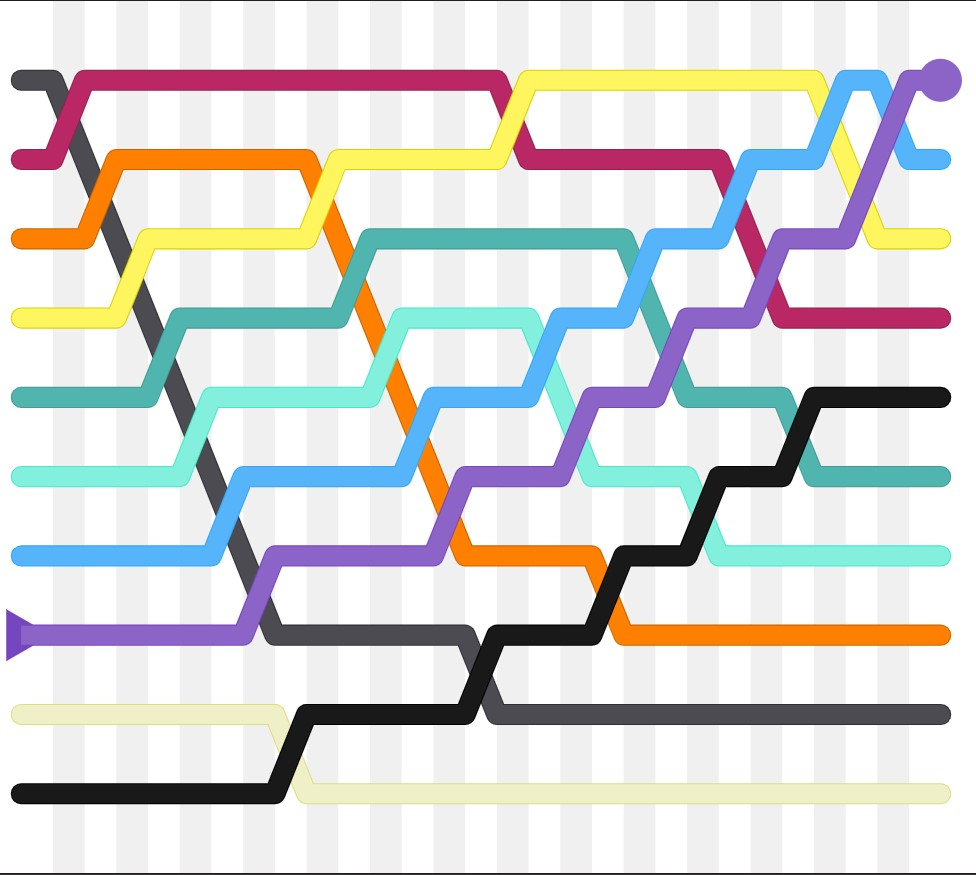
\includegraphics[height=4cm]{bubble.jpg} \caption{figure} asd
	%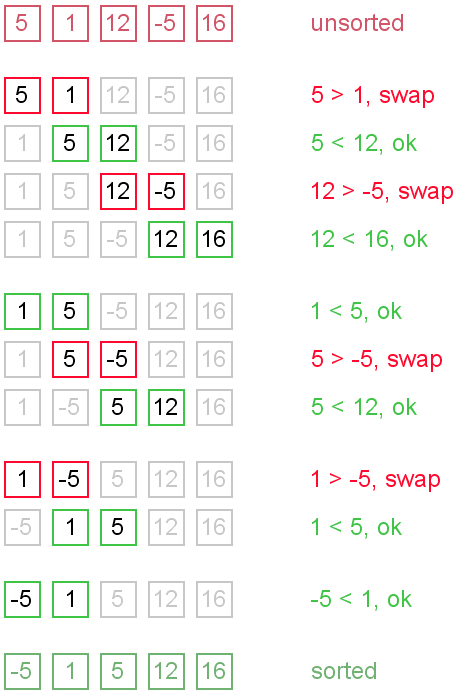
\includegraphics[height=4cm]{bubble-sort-1.png} \caption{fgdfgdfg}
	\begin{minipage}{0.49\linewidth}
		\begin{center}
			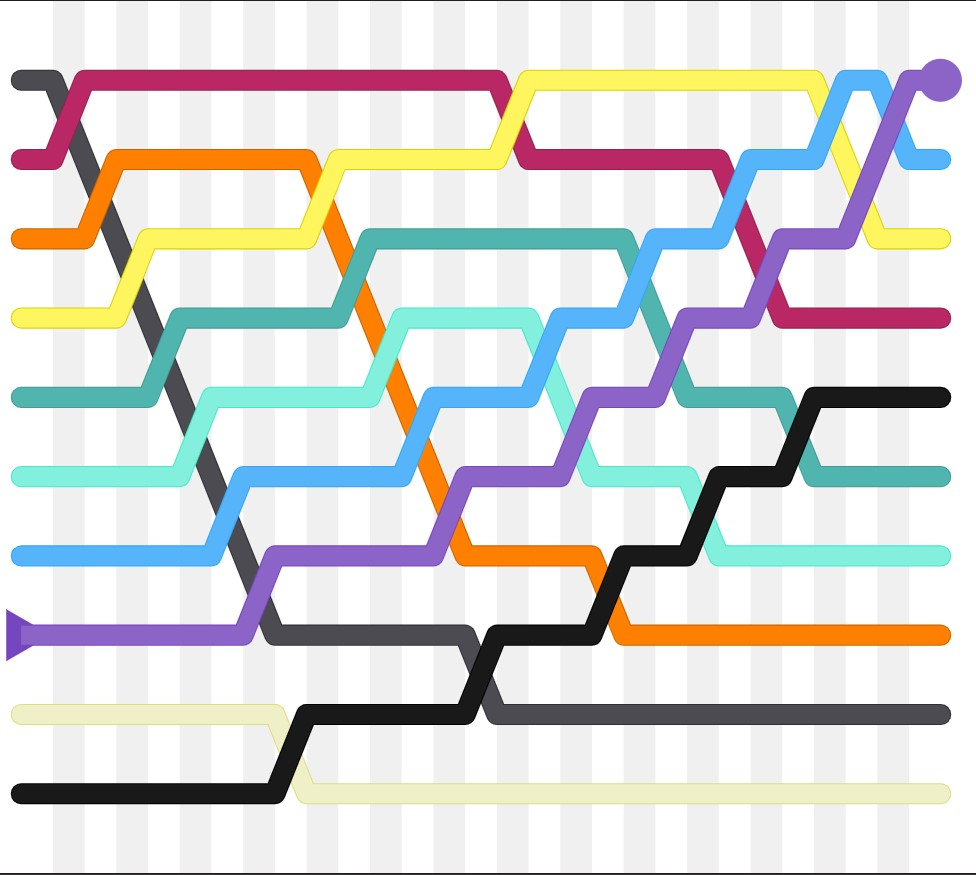
\includegraphics[height=4cm]{bubble.jpg}
			\captionof{figure}{Vizualizácia Bubble Sortu}
		\end{center}
	\end{minipage}
	\begin{minipage}{0.49\linewidth}
		\begin{center}
			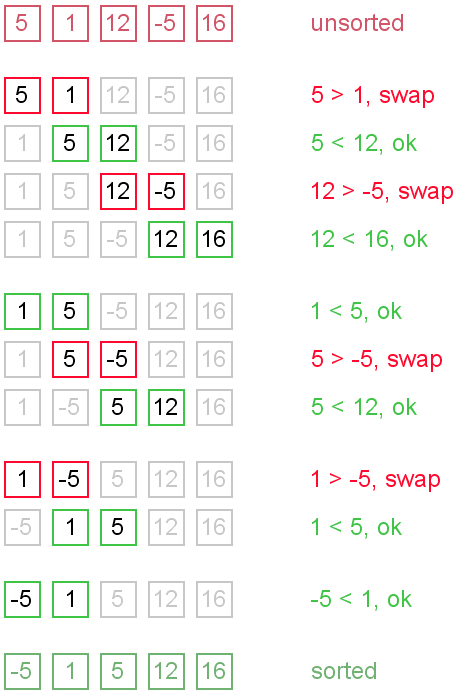
\includegraphics[height=4cm]{bubble-sort-1.png}
			\captionof{figure}{Príklad Bubble Sortu}
		\end{center}
	\end{minipage}

\end{center}
\end{frame}

%frame 6
\begin{frame}
\frametitle{Bubble Sort - algoritmus}
\IncMargin{1.5em}
\begin{algorithm}[H]
	\SetAlgoLined
	\SetInd{1em}{1em}
	\SetAlgoNlRelativeSize{-1}
	\SetNlSty{}{}{:}
	\SetNlSkip{0.4em}
	n = length(S)\;
	\While{n <= 1}{
		newn = 0\;
		\For{i = 1; i <= n-1; i++}{
			\If{S[i-1] > S[i]}{
				swap(S[i-1], S[i])\;
				newn = i;
			}
		}
		n = newn\;
	}
	
	\caption{Bubble Sort}
\end{algorithm}
\DecMargin{1.5em}
\end{frame}

%frame 7
\begin{frame}
\frametitle{Vlastnosti algoritmu Bubble Sort}
	\begin{itemize}
	\item Časová náročnosť
	\begin{itemize}
		\item Minimálna: $O(n)$
		\item Priemerná: $O(n^2)$
		\item Maximálna: $O(n^2)$
	\end{itemize}
	\item Pamäťová náročnosť
	\begin{itemize}
		\item $O(1)$
	\end{itemize}
	\item Prirodzenosť
	\begin{itemize}
		\item Áno
	\end{itemize}
	\item Stabilita
	\begin{itemize}
		\item Áno
	\end{itemize}
	\item Použitá metóda
	\begin{itemize}
		\item Zámena
	\end{itemize}
\end{itemize}
\end{frame}

\begin{frame}{Použité zdroje}
\begin{thebibliography}{8}
	\small
	\bibitem[Wikipedia]{Wikipedia} Řadící algoritmus
	\newblock  \texttt{https://cs.wikipedia.org/?curid=119181}
	
	\bibitem[Wikipedia]{Wikipedia} Bublinkové řazení
	\newblock \small \texttt{https://cs.wikipedia.org/?curid=158791}
	
	\bibitem[Wikipedia]{Wikipedia} Sorting algorithm
	\newblock \texttt{https://en.wikipedia.org/?curid=28442}
	
	\bibitem[Algolist]{Algolist} Bubble sort
	\newblock \texttt{http://www.algolist.net/Algorithms/Sorting/Bubble\_sort}
\end{thebibliography}
\end{frame}

\end{document}